```latex
\documentclass[12pt,a4paper]{article}
\usepackage[utf8]{inputenc}
\usepackage{amsmath}
\usepackage{amssymb}
\usepackage{xcolor}
\usepackage{tikz}
\usepackage{fancyhdr}
\usepackage[left=2.5cm,right=2.5cm,top=2.5cm,bottom=2.5cm]{geometry}

\newcommand{\bitstuff}[1]{\textcolor{red}{\textbf{#1}}}

\pagestyle{fancy}
\fancyhf{}
\rhead{Student ID: CN2024}
\lhead{Computer Networks Exam}
\rfoot{Page \thepage}

\begin{document}

\begin{center}
\Large\textbf{Computer Networks Examination}
\\\vspace{0.5cm}
\large\textit{Bit Stuffing Problem}
\end{center}

\section*{Question}
What would be the bit pattern of the following bit stream after "Bit Stuffing"? Please indicate the stuffed bit.

\begin{center}
\fbox{\texttt{0101011111101000000101111101}}
\end{center}

\section*{Solution}

\subsection*{1. Understanding Bit Stuffing}
Bit stuffing is a crucial technique in data link layer protocols to prevent pattern sensitivity. It involves inserting (or "stuffing") extra bits into the data stream to avoid the accidental occurrence of control sequences in the data.

\textbf{Key Rule:} In bit stuffing, a '0' bit is inserted after every sequence of five consecutive '1' bits.

\subsection*{2. Applying Bit Stuffing}
Let's analyze the given bit stream and apply bit stuffing:

\begin{center}
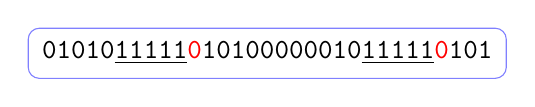
\begin{tikzpicture}
\node[draw=blue!50,rounded corners,inner sep=5pt] {
\texttt{01010\underline{11111}\bitstuff{0}10100000010\underline{11111}\bitstuff{0}101}
};
\end{tikzpicture}
\end{center}

\subsection*{3. Step-by-Step Process}
\begin{enumerate}
    \item \textbf{Initial scan:} We identify sequences of five consecutive '1' bits.
    \item \textbf{First occurrence:} After \texttt{01010\underline{11111}}
        \begin{itemize}
            \item Insert \bitstuff{0} $\rightarrow$ \texttt{0101011111\bitstuff{0}101000000101111101}
        \end{itemize}
    \item \textbf{Continue scanning:} Find the next sequence of five '1' bits
    \item \textbf{Second occurrence:} After \texttt{...010\underline{11111}}
        \begin{itemize}
            \item Insert \bitstuff{0} $\rightarrow$ \texttt{0101011111\bitstuff{0}101000000101111\bitstuff{0}101}
        \end{itemize}
    \item \textbf{Final scan:} No more sequences of five consecutive '1' bits remain.
\end{enumerate}

\subsection*{4. Resulting Bit Pattern}
The final bit pattern after bit stuffing is:

\begin{center}
\fbox{\texttt{0101011111\bitstuff{0}101000000101111\bitstuff{0}101}}
\end{center}

\textit{Note: The \textcolor{red}{\textbf{red}} bits indicate the stuffed bits.}

\subsection*{5. Verification}
To verify our solution, let's count the '1' bits between each '0' in the final pattern:
\[
\underbrace{01010}_5 \; \underbrace{11111}_5 \textcolor{red}{\textbf{0}} \; \underbrace{10100}_2 \; \underbrace{00001}_1 \; \underbrace{01111}_4 \textcolor{red}{\textbf{0}} \; \underbrace{101}_2
\]
As we can see, there are no more than five consecutive '1' bits anywhere in the resulting stream.

\section*{Conclusion}
Through the process of bit stuffing, we have successfully modified the original bit stream to prevent any occurrences of more than five consecutive '1' bits. This technique ensures that control sequences (typically 01111110) are not accidentally replicated within the data, maintaining the integrity of the frame structure in data link layer protocols.

\end{document}
```